%\chapter{Answers}
%% \chapter{Hints}
\graphicspath{{../07Implications/pics/}}

\chapter{Implications}\label{ch:Implications}
%\small
%\footnotesize

\subsubsection*{Exercise \ref{exe:carMakesSet}}

\begin{figure}[htbp]
  \centering
  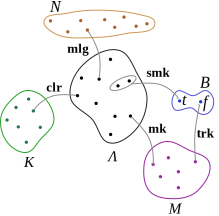
\includegraphics[scale=1.0]{diagramCars}
  \caption{The set $M$ contains all possible makes of cars: Ford,
    Toyota, etc.}
  \label{fig:diagramCars}
\end{figure}

The diagram in the Figure \ref{fig:diagramCars} shows the set $M$ -- the set
of all possible makes of cars. A mapping $\btc{trk}$ returns $true$ if a
given car maker produces trucks.

\subsubsection*{Exercise \ref{exe:relationsGeneral}}
\begin{figure}[htbp]
  \centering
  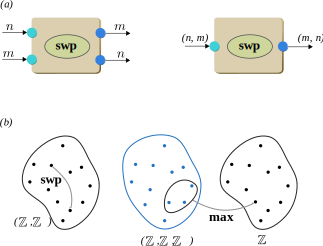
\includegraphics[scale=1.0]{diagramProductSet}
  \caption{(a) Two inputs (outputs) of a function can be replaced with
    a single input of a \bem{pair} of numbers, turning a binary
    function into a unary one. (b) That.}
  \label{fig:diagramProductSet}
\end{figure}

Any binary function can be viewed as a unary function
if two inputs are replaced by a single input of a \emph{pair of
numbers}. Similarly for a function with two outputs. This idea is
illustrated in the Figure \ref{fig:diagramProductSet}(a): The function
{\bf swp} is viewed as a unary function which swaps the numbers in an
\emph{ordered pair}:
\[
\textbf{ swp }\,(n,m) = (m, n)\,.
\]

Given the set $\mathbb{Z}$ of whole numbers, we can create the set of
all possible \emph{ordered pairs} $(n,m)$. This set can be denoted as
follows:
\[
(\mathbb{Z}, \mathbb{Z})\,\textrm{ or }\, \mathbb{Z}\times\mathbb{Z}\,.
\]

The latter notation is standard in mathematics, but the former way
of writing is also acceptable. We can similarly denote the set of all
\emph{ordered triples}:
\[
(\mathbb{Z}, \mathbb{Z}, \mathbb{Z})\,\textrm{ or }\, \mathbb{Z}\times\mathbb{Z}\times\mathbb{Z}\,.
\]

With the notation introduced above, the action of functions with
multiple inputs or outputs can be depicted on the level of sets. The
 Figure \ref{fig:diagramProductSet}(b) shows how this works for the
 functions $\textbf{ swp }$ and $\textbf{ max }$.

\subsubsection*{Exercise \ref{exe:binaryYourOwn}}
Consider a binary function that accepts a pair of natural numbers and
returns the third natural number in the following way:
\[
\textbf{ rep }\, 3\,2 = 33\,\quad\textbf{ rep }\, 1\,4 = 1111\,.
\]
Thus, the output is a natural number with identical digits given by
the first number, repeated a number of times specified by the second
number.

Infix variant of this operation can be written, rather arbitrarily,
like this:
\[
\textbf{ rep }\, n\,m = n\,\rightY\,m = nnn\ldots n\,.
\]

\subsubsection*{Exercise \ref{exe:linearFunctionSimple}}
A linear function $f$ must satisfy the linearity condition
\[
f\,(a*n)=a*(f\, n)\,.
\]
For $a=0$ we must have
\[
f\,(0*n)=0*(f\, n)\,,
\]
or, equivalently
\[
f\,0= 0\,.
\]

Also, for $a=m$ and $n=1$ we must have
\[
f\,(m*1)= m*(f\, 1)\,,
\]
from which follows
\[
f\,m= m(f\, 1)\,.
\]

\subsubsection*{Exercise \ref{exe:schematicLinearFunction}}
\begin{figure}[htbp]
  \centering
  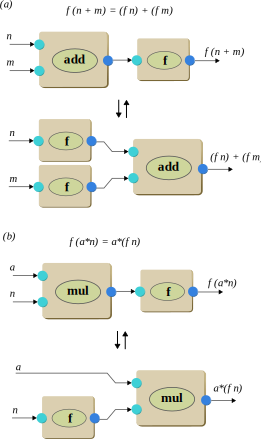
\includegraphics[scale=1.0]{schematicLinearFunction}
  \caption{The linearity conditions can be represented schematically
    with different relative configurations (order) of the ``boxes''.}
  \label{fig:schematicLinearFunction}
\end{figure}
The schematics in the Figure \ref{fig:schematicLinearFunction}(a) and
(b) demonstrate the two linearity requirements.

\subsubsection*{Exercise \ref{exe:polynomialESR}}
Using Einstein's summation
rule, a polynomial of degree $n$ can be written  as follows:
\[
P_n\, x = a_i x^i\,,\quad i=0,1,2\ldots,n\,.
\]

\subsubsection*{Exercise \ref{exe:dummyIndex}}
The expression
\[
b_iy_i\,,\quad i = 1,2,3,4
\]
represents the sum of four terms:
\[
S = b_1y_1 + b_2y_2 + b_3y_3 + b_4y_4\,.
\]

Similarly,
\[
b_jy_j\,,\quad j = 1,2,3,4
\]
stands for the same sum $S$, just as the expression
\[
b_ky_k = b_1y_1 + b_2y_2 + b_3y_3 + b_4y_4\,.
\]

\subsubsection*{Exercise \ref{exe:esrProduct}}
In the expression
\[
(a_ix_i)(a_jx_j)
\]
both parentheses contain the identical sum:
\[
a_ix_i = a_jx_j = a_1x_1 + a_2x_2\,.
\]
Opening the parentheses, we obtain
\[
(a_ix_i)(a_jx_j) = a^2_1x^2_1 + a^2_2x^2_2 + 2a_1a_2x_1x_2\,.
\]
In contrast, the expression $a_i^2x_i^2$ stands for
\[
a_i^2x_i^2 = a^2_1x^2_1 + a^2_2x^2_2\,.
\]
Clearly,
\[
a_i^2x_i^2 \ne (a_ix_i)^2\,.
\]

\subsubsection*{Exercise \ref{exe:esrVsTraditional}}
The left-hand side of the expression
\[
(a_i x_i)^2 = \frac{b_j y_j}{c_k c_k}
\]
can be written as
\[
(a_i x_i)^2 = \left(\sum\limits_{i=1}^{i=N}a_ix_i\right)^2
\]
The right-hand side takes the form:
\[
\frac{b_j y_j}{c_k c_k} = \frac{\sum\limits_{j=1}^{j=N} b_j
  y_j}{\sum\limits_{k=1}^{k=N} c_k c_k}\,.
\]
Therefore, the original equality can be re-written using the
traditional summation sign:
\[
\left(\sum\limits_{i=1}^{i=N}a_ix_i\right)^2 = \frac{\sum\limits_{j=1}^{j=N} b_j
  y_j}{\sum\limits_{k=1}^{k=N} c_k c_k}\,.
\]
Already one can see the advantage of Einstein's summation rule.


\subsubsection*{Exercise \ref{exe:deltaIndexSub}}
The expression
\[
\delta_{1i}a_i\,,\quad i = 1,2,3,4
\]
represents the sum
\[
\delta_{11}a_1 + \delta_{12}a_2 + \delta_{13}a_3 + \delta_{14}a_4\,.
\]
The only non-zero term corresponds to $\delta_{11} = 1$, therefore
\[
\delta_{1i}a_i = a_1\,.
\]

Similarly, we have
\[
\delta_{3k}a_k\,,\quad k = 1,2,3,4
\]
representing
\[
\delta_{31}a_1 + \delta_{32}a_2 + \delta_{33}a_3 + \delta_{34}a_4 = \delta_{33}a_3\,.
\]
Consequently,
\[
\delta_{3k}a_k = a_3\,.
\]

Next,
\[
\epsilon_{1j}a_j = \epsilon_{11}a_1 + \epsilon_{12}a_2 +
\epsilon_{13}a_3 + \epsilon_{14}a_4
\]
can be simplified to
\[
\epsilon_{1j}a_j = a_2 + a_3 + a_4
\]
using the definition of $\epsilon_{ij}$.

Finally, the expression
\[
\epsilon_{3j}a_j = \epsilon_{31}a_1 + \epsilon_{32}a_2 +
\epsilon_{33}a_3 + \epsilon_{34}a_4
\]
is reduced to
\[
\epsilon_{3j}a_j = a_4 - a_1 - a_2\,.
\]

\subsubsection*{Exercise \ref{exe:deltaRelabel}}
The sum
\[
a_i + a_j
\]
can be rewritten using the facts $a_j=\delta_{ji}a_i$ and $\delta_{ij}=\delta_{ji}$:
\[
a_i + a_j = a_i + \delta_{ij}a_i = (1+\delta_{ij})a_i = (1+\delta_{ji})a_i\,.
\]

\subsubsection*{Exercise \ref{exe:ESRScalarVectorProduct}}
(a) The expression $\delta_{ij}a_ib_j$ can be simplified using the
fact $\delta_{ij}b_j=b_i$:
\[
\delta_{ij}a_ib_j = a_ib_i = a_1b_1 + a_2b_2\,.
\]
(b) Fully writing out $\epsilon_{ij}a_ib_j$ results in
\[
\epsilon_{11}a_1b_1 + \epsilon_{12}a_1b_2 + \epsilon_{21}a_2b_1 + \epsilon_{22}a_2b_2\,.
\]
From the definition of $\epsilon_{ij}$ follows that only the terms
with $i\ne j$ survive:
\[
\epsilon_{ij}a_ib_j = a_1b_2 - a_2b_1\,.
\]


\subsubsection*{Exercise \ref{exe:advancedDeltaEpsilonProduct}}
(a) Firstly, we can recall that when $\delta_{ij}$  is summed with a
vector $a_j$ it simply ``renames'' the index that is being used for
summation:
\[
\delta_{ij}a_j = a_i\,.
\]
Using this property, we immediately get
\[
\delta_{ij}\delta_{jk} = \delta_{ik}\,.
\]
Another -- and longer -- way to get this result is to write out the
summation fully:
\[
\delta_{ij}\delta_{jk} = \delta_{i1}\delta_{1k} +
\delta_{i2}\delta_{2k} + \ldots + \delta_{in}\delta_{nk}\,.
\]
If $i\ne k$, all terms on the right are zero. Indeed,
$\delta_{i1}\delta_{1k}$ is zero unless $i=1$ and $k=1$; similarly,
$\delta_{i2}\delta_{2k}$ is zero unless $i=2$ and $k=2$ and so
on. Therefore, the only non-zero value for $\delta_{ij}\delta_{jk}$ is
when $i=k$. Let $i=k=m$, then in the sum
\[
\delta_{m1}\delta_{1m} +
\delta_{m2}\delta_{2m} + \ldots + \delta_{mm}\delta_{mm}+\ldots+\delta_{mn}\delta_{nm}\,.
\]
there is only one non-zero term, namely
\[
\delta_{mm}\delta_{mm} = 1\cdot 1 = 1\,.
\]
Summarizing the above arguments, we conclude that
\[
\delta_{ij}\delta_{jk} = 1\textrm{ if }i=k\textrm{ and } 0 \textrm{
  otherwise }\,.
\]
This is equivalent to the expression
\[
\delta_{ij}\delta_{jk} = \delta_{ik}\,.
\]
(b) The expression $\epsilon_{ij}\epsilon_{jk}$, when fully expanded
as a sum, takes the form
\[
\epsilon_{ij}\epsilon_{jk} = \epsilon_{i1}\epsilon_{1k} +
\epsilon_{i2}\epsilon_{2k}\,.
\]
If $i=k=1$, the sum is reduced to
\[
\epsilon_{1j}\epsilon_{j1} = \epsilon_{11}\epsilon_{11} +
\epsilon_{12}\epsilon_{21} = 1\cdot (-1) = -1\,.
\]
Similarly, for $i=k=2$ we get
\[
\epsilon_{2j}\epsilon_{j2} = \epsilon_{21}\epsilon_{12} +
\epsilon_{22}\epsilon_{22} = (-1)\cdot 1 = -1\,.
\]
On the other hand, if $i=1$ and $k=2$, we obtain
\[
\epsilon_{1j}\epsilon_{j2} = \epsilon_{11}\epsilon_{12} +
\epsilon_{12}\epsilon_{22} = 0\,.
\]
Same for $i=2$ and $k=1$:
\[
\epsilon_{2j}\epsilon_{j1} = \epsilon_{21}\epsilon_{11} +
\epsilon_{22}\epsilon_{21} = 0\,.
\]
We thus manually checked all cases and showed that
\[
\epsilon_{ij}\epsilon_{jk}=-\delta_{ik}\quad i,j,k=1,2\,.
\]


\subsubsection*{Exercise \ref{exe:ESRSymmetricAntisymmetric}}
Let us denote:
\[
x = \epsilon_{ij}a_ia_j\,.
\]
Since we can rename the summation indices, we can write
\[
\epsilon_{ij}a_ia_j = \epsilon_{ik}a_ia_k = \epsilon_{jk}a_ja_k = \epsilon_{ji}a_ja_i\,.
\]
Now we have $\epsilon_{ji} = -\epsilon_{ij}$ and this leads to
\[
\epsilon_{ji}a_ja_i = -\epsilon_{ij}a_ia_j\,.
\]
We thus showed that $x=-x$ and therefore $x=0$.


\subsubsection*{Exercise \ref{exe:ESRBasisExpansion}}
An expansion of an arbitrary vector $\vec{a}$ in terms of the basis
vectors is given by
\[
\vec{a} = a_1\vec{e}_1+a_2\vec{e}_2+a_3\vec{e}_3+\ldots a_n\vec{e}_n\,.
\]
This can be compactly written using Einstein's summation rule:
\[
\vec{a} = a_i\vec{e}_i\quad i=1,2,\ldots, n\,.
\]
If the number of basis vectors is known and fixed, as is usually the
case, we can omit the range of the summation index and simply write
\[
\vec{a} = a_i\vec{e}_i\,.
\]

\subsubsection*{Exercise \ref{exe:ESRBasesNewOld}}
The expression
\[
\vecp{e}_{1}=E_{11}\vec{e}_{1}+E_{12}\vec{e}_{2}\,,
\]
can be written using Einstein's summation rule as follows:
\[
\vecp{e}_{1}=E_{1j}\vec{e}_{j}\,.
\]

Similarly for the second basis vector:
\[
\vecp{e}_{2}=E_{2j}\vec{e}_{j}\,.
\]
Combining both results, we obtain
\[
\vecp{e}_i = E_{ij} \vec{e}_j\,.
\]

\subsubsection*{Exercise \ref{exe:contravariantExample1}}
(a) Writing the expansion of the ``new'' basis as follows:
\[
\vecp{e}_1 = \mu \vec{e}_{1} + 0\vec{e}_2\,,
\]
\[
\vecp{e}_2 = 0 \vec{e}_{1} + \nu\vec{e}_2\,,
\]
we can immediately find the components $E_{ij}$:
\[
E_{11} = \mu,\,E_{12} = 0,\,E_{21} = 0,\,E_{22} = \nu\,.
\]
We note that the ``new'' basis vectors are simply scaled version of
the ``old'' ones: $\vecp{e}_i$ is parallel to $\vec{e}_i$ but may have
different length (if $\mu,\nu \ne 1$).
(b) The simple relations between the ``new'' and ``old'' basis vectors
allow us to find
\[
\vec{e}_1 = \vecp{e}_{1} / \mu
\]
and
\[
\vec{e}_2 = \vecp{e}_2 / \nu\,.
\]
If the vector $\vec{a}$ is expanded using the ``old'' basis:
\[
\vec{a} = a_1\vec{e}_1 + a_2\vec{e}_2\,,
\]
then we can write
\[
\vec{a} = (a'_1/\mu)\vecp{e}_1 + (a'_2/\nu)\vecp{e}_2\,,
\]
and immediately find
\[
a'_1 = a_1/\mu\,,\quad a'_2 = a_2/\nu\,.
\]
Therefore, when the ``new'' basis vectors are scaled by factors $\mu$
and $\nu$, the corresponding ``new'' components of the vectors are
scaled by $1/\mu$ and $1/\nu$ -- \emph{in the opposite direction}, to
counter the effect of basis variation. The arrow-like vectors are thus called
\emph{contravariant vectors}.

\subsubsection*{Exercise \ref{exe:EEprimeExplicit}}
The compact expression
\[
E'_{ij}E_{jk}
\]
for $i=1$ and $k=2$ can be expanded into a sum:
\[
E'_{1j}E_{j2} = E'_{11}E_{12}+E'_{12}E_{22}\,.
\]

\subsubsection*{Exercise \ref{exe:InverseE}}
The system of four equations
\begin{eqnarray}
  aw + cx & = & 1\,,\\
  bw + dx & = & 0\,,\\
  ay + cz & = & 0\,,\\
  by + dz & = & 1
\end{eqnarray}
can be solved by noticing that the first two equations do not involve
the unknowns from the second pair of equations, and vice versa.

From the equation
\[
bw + dx =  0
\]
we first find $w = -dx/b$ and substitute in into the first equation:
\[
-adx/b + cx = 1\,,
\]
from which we easily find
\[
x = \frac{b}{cb-ad} = -\frac{b}{\Delta}\,,
\]
where we introduced the notation $\Delta = ad-bc$.
Then
\[
w = -\frac{dx}{b} = \frac{d}{\Delta}\,.
\]

The second pair of equations can be solved similarly. First, we get
\[
z = -\frac{ay}{c}\,,
\]
and substitute it into the last of four equations:
\[
by -\frac{ady}{c} = 1\,.
\]
From the last expression follows
\[
y = -\frac{c}{\Delta}\,.
\]
Consequently,
\[
z = \frac{a}{\Delta}\,.
\]

\subsubsection*{Exercise \ref{exe:inverseEDifferent}}
Firstly, we start with the compact expression
\[
E_{ij}E'_{jk} = \delta_{ik}
\]
and write it out fully for all four combinations of the indices $i$
and $k$:
\begin{eqnarray*}
  E_{11}E'_{11} + E_{12}E'_{21} & = & 1\,,\\
  E_{11}E'_{12} + E_{12}E'_{22} & = & 0\,,\\
  E_{21}E'_{11} + E_{22}E'_{21} & = & 0\,,\\
  E_{21}E'_{12} + E_{22}E'_{22} & = & 1\,.
\end{eqnarray*}

Secondly, using the notation
\[
E_{11} = a\,,\quad E_{12} = b\,,\quad E_{21} = c\,,\quad E_{22} = d\,,
\]
and
\[
E'_{11} = w\,,\quad E'_{12} = x\,,\quad E'_{21} = w\,,\quad E'_{22} = z\,,
\]
we arrive at the four equations which we can group into two pairs of
equations, each pair involves only two unknowns. The first pair is
\begin{eqnarray*}
  aw + by & = & 1\,,\\
  cw + dy & = & 0\,;
\end{eqnarray*}
the second pair:
\begin{eqnarray*}
  cx + dz & = & 1\,,\\
  ax + bz & = & 0\,.
\end{eqnarray*}

The first pair is easily solved when we find
\[
w = -\frac{dy}{c}\,,
\]
and substitute it into the first equation of the first pair:
\[
-\frac{ady}{c}+by = 1\,,
\]
from which follows:
\[
y = -\frac{c}{\Delta}\,\quad \Delta = ad - bc\,.
\]
Immediately we get
\[
w = \frac{d}{\Delta}\,.
\]
Similarly, we first find
\[
z = -\frac{ax}{b}\,,
\]
and substitute into the first equation of the second pair:
\[
cx -\frac{adx}{b} = 1\,.
\]
Solving for $x$, we get
\[
x = \frac{b}{\Delta}\,,
\]
and therefore
\[
z = \frac{a}{\Delta}\,.
\]

We conclude that although two conditions $E'_{ij}E_{jk} = \delta_{ik}$ and
$E_{ij}E'_{jk} = \delta_{ik}$ result in slightly different equations,
they put the same constraints on the relations between the coefficients
$E_{ij}\,(a,b,c,d)$ and $E'_{nm}\,(w,x,y,z)$.

\subsubsection*{Exercise \ref{exe:CircleToParabola}}
The equation of a circle with the radius $R$ can be written using
Cartesian coordinates:
\[
x^2 + y^2 = R^2\,.
\]
The transformation
\[
b_1 = a_1 + a_2\,,\quad b_2 = a_1 * a_2
\]
moves every point $(x,y)$ into a new point $(x', y')$ related by the
same equations:
\[
x' = x + y\,,\quad y' = xy\,.
\]
Squaring $x'$, we get
\[
(x')^2 = x^2 + y^2 + 2xy = R^2 + 2y'\,.
\]
Therefore, the components of the transformed vector are related as
follows:
\[
y' = (x')^2/2 - R^2/2\quad\Leftrightarrow\quad b_2 = b_1^2/2 - R^2/2\,.
\]

%% \subsubsection*{Exercise \ref{exe:scalingTransformation}}
%% Using the polar coordinates
%% \[
%% a_1 = R \cos\theta\,,\qquad a_2 = R\sin\theta\,,
%% \]
%% the transformed coordinates become
%% \[
%% b_1 = R(\cos\theta -\sin\theta)\,,
%% \]
%% \[
%% b_2 = -R^3\cos^2\theta * |\sin\theta|\,.
%% \]
%% Clearly, $b_1$ scales linearly with the magnitude of
%% $|a_1|=R$, while $b_2$ grows as the third power.

\subsubsection*{Exercise \ref{exe:normalizationOperator}}
The operator of normalization $\op{N}$ fails to satisfy the first
linearity condition because
\[
\op{N}\,(\alpha \vec{a}) \ne \alpha (\op{N}\,\vec{a})\,.
\]
Indeed, the left-hand side must be a unit vector in the direction of
$\alpha\vec{a}$, which is the same as the direction of $\vec{a}$:
\[
\op{N}\,(\alpha \vec{a}) = \vec{u}_a = \op{N}\,\vec{a}\,.
\]
In addition, the operator $\op{N}$ does not satisfy the second
linearity condition:
\[
\op{N}\,(\vec{a}+\vec{b}) = (\op{N}\,\vec{a}) + (\op{N}\,\vec{b})\,.
\]
Take, for instance, $\vec{a}=\vec{e}_1$ and
$\vec{b}=1000\vec{e}_2$. The sum-vector $\vec{a}+\vec{b}$ will be
pointing almost along the second basis vector $\vec{e}_2$, therefore
\[
\op{N}\,(\vec{e}_1+1000\vec{e}_2)
\]
will be a unit vector \emph{almost parallel} to $\vec{e}_2$. However,
the vector
\[
(\op{N}\,\vec{e}_1) + (\op{N}\,[1000\vec{e}_2]) = \vec{e}_1 + \vec{e}_2
\]
will go diagonally between $\vec{e}_1$ and $\vec{e}_2$.


\subsubsection*{Exercise \ref{exe:degenerateCollapse}}
The condition for degeneracy of a linear operator can be written as follows:
\[
\op{L}\,\vec{e}_1 = \lambda\left(\op{L}\,\vec{e}_2\right)\,.
\]
For simplicity, let us denote $\vec{v} = \op{L}\,\vec{e}_2$. Then we
have
\[
\op{L}\,\vec{e}_1 = \lambda \vec{v}\,.
\]

For an arbitrary vector $\vec{a}$ we can find the action of the
degenerate linear operator $\op{L}$
\[
\op{L}\,\vec{a} = \op{L}\,(a_1\vec{e}_1 + a_2\vec{e}_2) = a_1
(\op{L}\,\vec{e}_1) + a_2(\op{L}\,\vec{e}_2)\,.
\]
Now we can use the degeneracy condition to find
\[
\op{L}\,\vec{a} = a_1\lambda \vec{v}+a_2\vec{v} = (a_1\lambda +
a_2)\vec{v}=\alpha \vec{v}\,.
\]
Thus, any vector is mapped into a vector parallel to $\vec{v}$. In
other words, degenerate linear operator ``collapses'' all vectors onto
a single line.


\subsubsection*{Exercise \ref{exe:vectorComponentsCovariance}}
The relation
\[
\op{L}\,\vec{a} = \vec{b}
\]
can be written using components relative to the ``new'' basis
$\lbrace \vecp{e}_i\rbrace$. Expanding the vector $\vec{a}$, we get:
\[
\op{L}\,(a'_i\vecp{e}_i) = a'_i(\op{L}\,\vecp{e}_i)\,.
\]
Now the components of the operator $\op{L}$ relative to the ``new''
basis are defined similarly to the components relative to the ``old''
basis:
\[
\op{L}\,\vecp{e}_i = L'_{ij}\vecp{e}_j\,.
\]
Combining the last two expressions, we obtain
\[
\op{L}\,\vec{a} = (a'_iL'_{ij})\vecp{e}_j\,,
\]
where we indicated that the summation with the components of the
vector $\vec{a}$ happens first. Comparing this result with the
expansion of the vector $\vec{b}$ relative to the ``new'' basis
\[
\vec{b} = b'_j\vecp{e}_j\,,
\]
we can see that the following relation holds
\[
a'_iL'_{ij} = b'_j\,.
\]

\subsubsection*{Exercise \ref{exe:traceInvariance}}
To evaluate the right-hand side of the expression
\[
L_{11} +L_{22} = L'_{11} + L'_{22}\,,
\]
we need to recall to rule of transformation of components of the
linear operator:
\[
L'_{mj} = E_{mk}L_{ki}E'_{ij}\,.
\]
Using the last expression we can write
\[
L'_{11} = E_{1k}L_{ki}E'_{i1} = (E'_{i1}E_{1k}) L_{ki}
\]
and
\[
L'_{22} = E_{2k}L_{ki}E'_{i2} = (E'_{i2}E_{2k}) L_{ki}\,.
\]
Summing up, we obtain
\[
L'_{11} + L'_{22} = \left(E'_{i1}E_{1k} +E'_{i2}E_{2k} \right)L_{ki}\,.
\]
The sum in the parentheses can be made more compact using Einstein's summation
rule:
\[
E'_{i1}E_{1k} +E'_{i2}E_{2k} = E'_{ij}E_{jk}\,.
\]
We showed that
\[
E'_{ij}E_{jk} = \delta_{ik}\,,
\]
therefore
\[
L'_{11} + L'_{22} = \delta_{ik}L_{ki}=L_{ii} = L_{11}+L_{22}\,.
\]

\subsubsection*{Exercise \ref{exe:angleOperatorNonlinear}}
The operator $\angle$ is not linear in either of its
arguments. Indeed, scaling the first argument by an arbitrary factor
$\alpha$ does not affect the measured angle:
\[
\angle\,(\alpha \vec{a})\,\vec{b} = \angle\, \vec{a}\,\vec{b} \ne
\alpha (\angle\, \vec{a}\,\vec{b})\,.
\]
Same applies to the second argument.

\subsubsection*{Exercise \ref{exe:projectorOperatorFromScalarProduct}}
Components of any linear operator are defined as the coefficients in
the expansion
\[
\op{L}\,\vec{e}_i = L_{ij}\vec{e}_j\,.
\]
For the potential operator $\op{\beta}$ this means
\[
\op{\beta}\,\vec{e}_i = (a_ib_j)\vec{e}_j = a_i(b_j\vec{e}_j) = a_i\vec{b}\,.
\]
Thus, the operator $\op{\beta}$ maps all basis vectors into vectors
parallel to $\vec{b} = b_j\vec{e}_j$. Consequently, the operator
$\op{\beta}$ maps \emph{all} vectors into the same direction parallel
to the vector $\vec{b}$. It is an example of a \emph{degenerate linear
operator}. See also {Exercise \ref{exe:degenerateCollapse}}.


\subsubsection*{Exercise \ref{exe:expansionInConjugateBasis}}
By definition
\[
\vecl{a} = \op{\sigma}\,\vec{a} = \op{\sigma}\,(a_1\vec{e}_1+a_2\vec{e}_2)\,.
\]
Using the linearity of $\op{\sigma}$, we first write
\[
\op{\sigma}\,(a_1\vec{e}_1+a_2\vec{e}_2) =
\lbrack\op{\sigma}\,(a_1\vec{e}_1)\rbrack +
\lbrack\op{\sigma}\,(a_2\vec{e}_2)\rbrack\,.
\]
Using the linearity again, we get
\[
\op{\sigma}\,(a_1\vec{e}_1)=a_1(\op{\sigma}\,\vec{e}_1) = a_1\vecl{e}_1
\]
and
\[
\op{\sigma}\,(a_2\vec{e}_2)=a_2(\op{\sigma}\,\vec{e}_2)=a_2\vecl{e}_2\,,
\]
which lead to
\[
\vecl{a}=\op{\sigma}\,(a_1\vec{e}_1+a_2\vec{e}_2) = a_i\vecl{e}_i\,.
\]
We showed that vector conjugate to $\vec{a}$ can be expanded in terms
of basis conjugate to $\vec{e}_i$.

\subsubsection*{Exercise \ref{exe:determinantOfProjector}}
The determinant of a linear operator $\op{L}$ can be calculated from
its components according to:
\[
det\,\op{L} = L_{11}L_{22}-L_{12}L_{21}\,.
\]
For a projector $\projop{A}$ we have
\[
\proj{A}_{11}\proj{A}_{22} = \frac{a_1a_1a_2a_2}{a^4}
= \frac{a_1^2a_2^2}{a^4}
\]
and
\[
\proj{A}_{12}\proj{A}_{21} = \frac{a_1a_2a_2a_1}{a^4}
= \frac{a_1^2a_2^2}{a^4}\,.
\]
It immediately follows that $det\,\op{L}=0$.

A helpful related exercise is Exercise \ref{exe:projectorOperatorFromScalarProduct}.

\subsubsection*{Exercise \ref{exe:projectorIdempotent}}
(a) First, we can write symbolically:
\[
\projop{A}\circ \projop{A} =
\frac{(\vec{a}\vecl{a})}{a^2}\frac{(\vec{a}\vecl{a})}{a^2} =
\frac{\vec{a}(\vecl{a}\vec{a})\vecl{a}}{a^4}\,,
\]
which, using the fact  $\vecl{a}\vec{a}=a^2$ is reduced to
\[
\projop{A}\circ \projop{A} =
\frac{\vec{a}\vecl{a}}{a^2}=\projop{A}\,.
\]

Second, using components, we write the product of two operators as
follows:
\[
(\proj{A}_{ij})(\proj{A}_{jk}) = \frac{a_ia_ja_ja_k}{a^4}\,.
\]
Recalling that $a_ja_j = a^2$, we find
\[
(\proj{A}_{ij})(\proj{A}_{jk}) = \frac{a_ia_k}{a^2}=\proj{A}_{ik}\,.
\]
Every projector of the type $L=\vec{d}\vecl{d}/d^2$ has this property.

(b) For a composition of two projectors
\[
\op{L}=\projop{B}\circ \projop{A}
\]
the components are given by
\[
L_{ik} = \lambda\, a_ib_k,\quad \lambda = \frac{\vec{a}\cdot\vec{b}}{a^2b^2}\,.
\]
Composition of two such operators can be evaluated using their components:
\[
L_{ik}L_{kj} = (\lambda\, a_ib_k)(\lambda\, a_kb_j) = \lambda^2
a_i(a_kb_k)b_j = \lambda^2 (\vec{a}\cdot\vec{b})a_ib_j\,.
\]
We thus showed that
\[
\op{L}\circ\op{L} = \lambda (\vec{a}\cdot\vec{b})\op{L}\,.
\]
Now
\[
\lambda (\vec{a}\cdot\vec{b}) = \frac{(\vec{a}\cdot\vec{b})^2}{a^2b^2}
= \cos\theta\,,
\]
where $\theta$ is the angle between the vectors $\vec{a}$ and
$\vec{b}$. Therefore,
\[
\op{L}\circ\op{L} = \cos\theta\op{L}\ne\op{L}\,.
\]
Only for $\vec{a}=\vec{b}$ we have the property $\op{L}\circ\op{L} = \op{L}$.

\subsubsection*{Exercise \ref{exe:projectorsCommutativity}}
The components of the composition
\[
\op{L}=\projop{B}\circ \projop{A}\,.
\]
are
\[
L_{ik} = \lambda\, a_ib_k,\quad \lambda = \frac{\vec{a}\cdot\vec{b}}{a^2b^2}\,.
\]
Reversing the order of arguments of the composition results in
\[
\op{M}=\projop{A}\circ \projop{B}\,,
\]
with the components
\[
M_{ik} = \lambda\, b_ia_k,\quad \lambda = \frac{\vec{b}\cdot\vec{a}}{a^2b^2}\,.
\]
In general, $M_{12} \ne L_{12}$ because $a_1b_2\ne b_1a_2$.

\subsubsection*{Exercise \ref{exe:transformation4Kinds}}
To arrive at the transformation rules for the components of different
types of tensors, we will use a simple fact: A general tensor with
components $t^{ij}$ will behave just like the tensor product of two
contra-variant vectors $a^ib^j$. Thus, we will study four types of
tensor products:
\[
a^ib^j\,,\quad a_ib_j\,,\quad a^ib_j\,,\quad a_ib^j\,.
\]

It will be helpful to recall the transformation rules of
contravariant and covariant vectors. An arrow-like contravariant
vector can be expanded in a basis:
\[
\vec{a}=a^i\vec{e}_i\,.
\]
Every vectors from a ``new'' basis can be similarly expanded:
\[
\vecp{e}_j = E_{j\tus}^{\tus k}\vec{e}_k\,.
\]
Here we deliberately included the ``dummy'' symbol ``$\tus$'' to
visually align the indices according to their order.
Expanding the same vector $\vec{a}$ relative to the ``new'' basis has
the form:
\[
\vec{a}=a'^i\vecp{e}_i\,,
\]
and similarly
\[
\vec{a}=a^i\vec{e}_i\,.
\]\[
\vec{e}_k = (E')_{k\tus}^{\tus j}\vec{e}_j\,.
\]
We also obtained the relation between the components of the same
vector $\vec{a}$ in different bases:
\[
a'^i = (E')_{k\tus}^{\tus i}a^k\,.
\]
Another contravariant vector will have similar relations:
\[
b'^j = (E')_{l\tus}^{\tus j}b^l\,,
\]
and their tensor product $t^{ij} = a^ib^j$ will be transformed
according to
\[
(t')^{ij} = (E')_{k\tus}^{\tus i}(E')_{l\tus}^{\tus j}t^{kl}\,.
\]

Using the transformation rule of covariant components:
\[
a'_i = E_{i\tus}^{\tus k}a_k\quad\textrm{ and }\quad
b'_j = E_{j\tus}^{\tus l}a_l\,,
\]
we immediately arrive at transformation rule of the components of a
doubly-covariant tensor:
\[
t'_{ij} = E_{i\tus}^{\tus k}E_{j\tus}^{\tus l}t_{kl}\,.
\]
In a similar fashion, by combining the transformation rules of
contravariant and covariant vectors, we can obtain the transformation
of contra-covariant tensor:
\[
(t')^{i\tus}_{\tus j} = (E')_{k\tus}^{\tus i} E_{j\tus}^{\tus l} t^{k\tus}_{\tus l}\,,
\]
and covariant-contravariant tensor:
\[
(t')_{i\tus}^{\tus j } = E_{i\tus}^{\tus k}(E')_{l\tus}^{\tus j}t_{k\tus}^{\tus l}\,.
\]

\subsubsection*{Exercise \ref{exe:metricTensorScalarProduct}}
(a) The action of the metric tensor on a tensor product
$\vec{a}\otimes\vec{b}$ can be understood once we write it out using
components. First, let's write the expression for the distance squared:
\[
d^2 = \eta_{ij}d^id^j\,.
\]
In a similar way, we can write
\[
\op{\eta}\,(\vec{a}\otimes\vec{b}) = \eta_{ij}a^ib^j\,.
\]
Using the fact
\[
\eta_{ij} = \op{\sigma}\,\vec{e}_i\,\vec{e}_j
\]
and bilinear nature of the dol-operator $\op{\sigma}$, we deduce
\[
\eta_{ij}a^ib^j =
a^ib^j(\op{\sigma}\,\vec{e}_i\,\vec{e}_j)=
\op{\sigma}\,(a^i\vec{e}_i)\,(b^j\vec{e}_j)=
\op{\sigma}\vec{a}\,\vec{b}\,.
\]
Thus, we showed that
\[
\op{\eta}\,(\vec{a}\otimes\vec{b}) = \vec{a}\cdot\vec{b}\,.
\]
The connection between the metric tensor and scalar products is not
surprising. Indeed, if we recall that if vector $\vec{d}$ connects two
points in a plane and is given by
\[
\vec{d} = \vec{b} - \vec{a}\,,\quad d^i = b^i - a^i\,,
\]
then
\[
\eta_{ij}d^id^j = \eta_{ij}(a^i-b^i)(a^j-b^j) = \eta_{ij}a^ia^j+\eta_{ij}b^ib^j+2\eta_{ij}a^ib^j\,.
\]
We arrived at the familiar theorem of planar geometry -- theorem of
cosine:
\[
d^2 = a^2 + b^2 - 2ab\cos\theta\,.
\]
(b) Vectors of orthonormal basis all have unit lengths
(\emph{normalized} vectors):
\[
e_i^2 = \op{\sigma}\, \vec{e}_i\,\vec{e}_i = \eta_{ii} = 1\,.
\]
Different vectors of orthonormal basis are perpendicular to each other
(\emph{orthogonal} vectors):
\[
\vec{e}_i\cdot\vec{e}_j = \op{\sigma}\, \vec{e}_i\,\vec{e}_j = \eta_{ij} = 0\,.
\]
We showed that
\[
\eta_{ij} = \delta_{ij}
\]
when the basis is orthonormal.
